\documentclass[10pt,a4paper]{article}\usepackage[]{graphicx}\usepackage[]{color}
%% maxwidth is the original width if it is less than linewidth
%% otherwise use linewidth (to make sure the graphics do not exceed the margin)
\makeatletter
\def\maxwidth{ %
  \ifdim\Gin@nat@width>\linewidth
    \linewidth
  \else
    \Gin@nat@width
  \fi
}
\makeatother

\definecolor{fgcolor}{rgb}{0.345, 0.345, 0.345}
\newcommand{\hlnum}[1]{\textcolor[rgb]{0.686,0.059,0.569}{#1}}%
\newcommand{\hlstr}[1]{\textcolor[rgb]{0.192,0.494,0.8}{#1}}%
\newcommand{\hlcom}[1]{\textcolor[rgb]{0.678,0.584,0.686}{\textit{#1}}}%
\newcommand{\hlopt}[1]{\textcolor[rgb]{0,0,0}{#1}}%
\newcommand{\hlstd}[1]{\textcolor[rgb]{0.345,0.345,0.345}{#1}}%
\newcommand{\hlkwa}[1]{\textcolor[rgb]{0.161,0.373,0.58}{\textbf{#1}}}%
\newcommand{\hlkwb}[1]{\textcolor[rgb]{0.69,0.353,0.396}{#1}}%
\newcommand{\hlkwc}[1]{\textcolor[rgb]{0.333,0.667,0.333}{#1}}%
\newcommand{\hlkwd}[1]{\textcolor[rgb]{0.737,0.353,0.396}{\textbf{#1}}}%

\usepackage{framed}
\makeatletter
\newenvironment{kframe}{%
 \def\at@end@of@kframe{}%
 \ifinner\ifhmode%
  \def\at@end@of@kframe{\end{minipage}}%
  \begin{minipage}{\columnwidth}%
 \fi\fi%
 \def\FrameCommand##1{\hskip\@totalleftmargin \hskip-\fboxsep
 \colorbox{shadecolor}{##1}\hskip-\fboxsep
     % There is no \\@totalrightmargin, so:
     \hskip-\linewidth \hskip-\@totalleftmargin \hskip\columnwidth}%
 \MakeFramed {\advance\hsize-\width
   \@totalleftmargin\z@ \linewidth\hsize
   \@setminipage}}%
 {\par\unskip\endMakeFramed%
 \at@end@of@kframe}
\makeatother

\definecolor{shadecolor}{rgb}{.97, .97, .97}
\definecolor{messagecolor}{rgb}{0, 0, 0}
\definecolor{warningcolor}{rgb}{1, 0, 1}
\definecolor{errorcolor}{rgb}{1, 0, 0}
\newenvironment{knitrout}{}{} % an empty environment to be redefined in TeX

\usepackage{alltt}

\usepackage[T1]{fontenc}
\usepackage[polish]{babel}
\usepackage[cp1250]{inputenc}
\usepackage{amsmath}
\usepackage{amsfonts}
\usepackage{graphicx}
\usepackage{setspace}
\usepackage{savesym}
\savesymbol{arc}
\usepackage{color}
\usepackage{xcolor}
\usepackage{pict2e}
\usepackage{epstopdf}
\usepackage{geometry}

\newgeometry{tmargin=0.9cm, bmargin=0.9cm, lmargin=0.9cm, rmargin=0.9cm}
\pagestyle{empty}
\linespread{1}
\IfFileExists{upquote.sty}{\usepackage{upquote}}{}

\begin{document}

\subsection*{Zadanie 1.1}

\begin{knitrout}
\definecolor{shadecolor}{rgb}{0.969, 0.969, 0.969}\color{fgcolor}\begin{kframe}
\begin{alltt}
\hlcom{# 1.1}

\hlstd{e} \hlkwb{<-} \hlkwd{read.table}\hlstd{(}\hlstr{"http://www.ipipan.eu/~teisseyrep/TEACHING/DM/DANE/earthquake.txt"}\hlstd{,}
    \hlkwc{header} \hlstd{=} \hlnum{TRUE}\hlstd{)}
\hlkwd{head}\hlstd{(e)}
\end{alltt}
\begin{verbatim}
##     popn body surface
## 1 equake 5.60    4.25
## 2 equake 5.18    3.93
## 3 equake 6.31    6.30
## 4 equake 5.36    4.49
## 5 equake 5.96    6.39
## 6 equake 5.26    4.42
\end{verbatim}
\begin{alltt}
\hlkwd{attach}\hlstd{(e)}

\hlcom{# a)}

\hlstd{n} \hlkwb{<-} \hlkwd{nrow}\hlstd{(e)}
\hlstd{ile} \hlkwb{<-} \hlkwd{table}\hlstd{(popn)}
\hlstd{ile}
\end{alltt}
\begin{verbatim}
## popn
##  equake explosn 
##      20       9
\end{verbatim}
\begin{alltt}
\hlstd{nq} \hlkwb{<-} \hlstd{ile[}\hlnum{1}\hlstd{]}
\hlstd{nx} \hlkwb{<-} \hlstd{ile[}\hlnum{2}\hlstd{]}

\hlstd{kol} \hlkwb{<-} \hlkwd{c}\hlstd{(}\hlkwd{rep}\hlstd{(}\hlstr{"red"}\hlstd{, nq),} \hlkwd{rep}\hlstd{(}\hlstr{"blue"}\hlstd{, nx))}
\hlstd{styl} \hlkwb{<-} \hlkwd{c}\hlstd{(}\hlkwd{rep}\hlstd{(}\hlstr{"Q"}\hlstd{, nq),} \hlkwd{rep}\hlstd{(}\hlstr{"X"}\hlstd{, nx))}

\hlkwd{plot}\hlstd{(body, surface,} \hlkwc{col} \hlstd{= kol,} \hlkwc{pch} \hlstd{= styl,} \hlkwc{cex} \hlstd{=} \hlnum{0.5}\hlstd{)}
\end{alltt}
\end{kframe}

{\centering 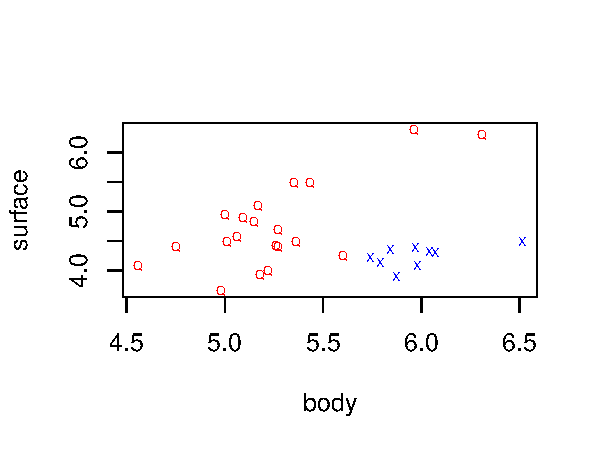
\includegraphics[width=\maxwidth]{figure/unnamed-chunk-1} 

}



\end{knitrout}


\begin{knitrout}
\definecolor{shadecolor}{rgb}{0.969, 0.969, 0.969}\color{fgcolor}\begin{kframe}
\begin{alltt}
\hlcom{# b)}

\hlcom{# macierze kowariancji w klasach:}

\hlstd{eq} \hlkwb{<-} \hlstd{e[popn} \hlopt{==} \hlstr{"equake"}\hlstd{, ]}
\hlstd{ex} \hlkwb{<-} \hlstd{e[popn} \hlopt{==} \hlstr{"explosn"}\hlstd{, ]}

\hlstd{(cov_q} \hlkwb{<-} \hlkwd{cov}\hlstd{(eq[,} \hlnum{2}\hlopt{:}\hlnum{3}\hlstd{]))}
\end{alltt}
\begin{verbatim}
##           body surface
## body    0.1478   0.200
## surface 0.2000   0.527
\end{verbatim}
\begin{alltt}
\hlstd{(cov_x} \hlkwb{<-} \hlkwd{cov}\hlstd{(ex[,} \hlnum{2}\hlopt{:}\hlnum{3}\hlstd{]))}
\end{alltt}
\begin{verbatim}
##            body surface
## body    0.05226 0.02346
## surface 0.02346 0.03253
\end{verbatim}
\begin{alltt}
\hlcom{# macierz kowariancji wewnatrzgrupowej:}

\hlstd{(w} \hlkwb{<-} \hlstd{((nq} \hlopt{-} \hlnum{1}\hlstd{)} \hlopt{*} \hlstd{cov_q} \hlopt{+} \hlstd{(nx} \hlopt{-} \hlnum{1}\hlstd{)} \hlopt{*} \hlstd{cov_x)}\hlopt{/}\hlstd{(n} \hlopt{-} \hlnum{2}\hlstd{))}
\end{alltt}
\begin{verbatim}
##           body surface
## body    0.1195  0.1477
## surface 0.1477  0.3805
\end{verbatim}
\begin{alltt}
\hlcom{# pierwszy wektor kanoniczny:}

\hlstd{(sr_q} \hlkwb{<-} \hlkwd{apply}\hlstd{(eq[,} \hlnum{2}\hlopt{:}\hlnum{3}\hlstd{],} \hlnum{2}\hlstd{, mean))}
\end{alltt}
\begin{verbatim}
##    body surface 
##   5.249   4.740
\end{verbatim}
\begin{alltt}
\hlstd{(sr_x} \hlkwb{<-} \hlkwd{apply}\hlstd{(ex[,} \hlnum{2}\hlopt{:}\hlnum{3}\hlstd{],} \hlnum{2}\hlstd{, mean))}
\end{alltt}
\begin{verbatim}
##    body surface 
##   5.979   4.244
\end{verbatim}
\begin{alltt}
\hlstd{(a} \hlkwb{<-} \hlkwd{solve}\hlstd{(w)} \hlopt \hlkwd{t}\hlstd{(}\hlkwd{t}\hlstd{(sr_x} \hlopt{-} \hlstd{sr_q)))}
\end{alltt}
\begin{verbatim}
##           [,1]
## body    14.832
## surface -7.059
\end{verbatim}
\begin{alltt}
\hlcom{# prosta rozdzielajaca klasy:}

\hlstd{z} \hlkwb{<-} \hlnum{1}\hlopt{/}\hlnum{2} \hlopt{*} \hlstd{(sr_x} \hlopt{+} \hlstd{sr_q)}

\hlstd{wsp_kier} \hlkwb{<-} \hlopt{-}\hlstd{a[}\hlnum{1}\hlstd{]}\hlopt{/}\hlstd{a[}\hlnum{2}\hlstd{]}
\hlstd{wyr_woln} \hlkwb{<-} \hlkwd{t}\hlstd{(a)} \hlopt \hlkwd{t}\hlstd{(}\hlkwd{t}\hlstd{(z))}\hlopt{/}\hlstd{a[}\hlnum{2}\hlstd{]}

\hlkwd{plot}\hlstd{(body, surface,} \hlkwc{col} \hlstd{= kol,} \hlkwc{pch} \hlstd{= styl,} \hlkwc{cex} \hlstd{=} \hlnum{0.5}\hlstd{)}
\hlkwd{abline}\hlstd{(wyr_woln, wsp_kier)}
\end{alltt}
\end{kframe}

{\centering 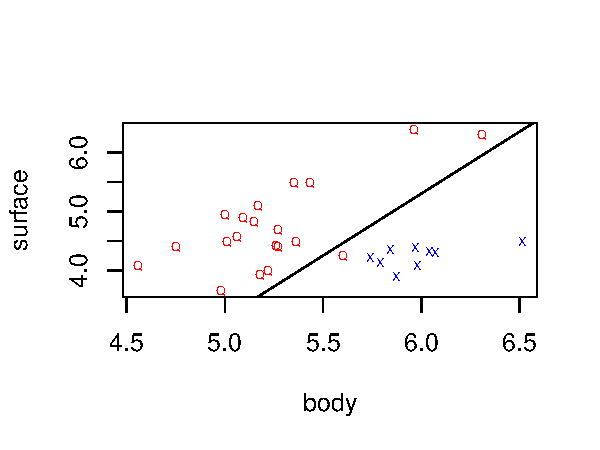
\includegraphics[width=\maxwidth]{figure/unnamed-chunk-2} 

}



\end{knitrout}


\begin{knitrout}
\definecolor{shadecolor}{rgb}{0.969, 0.969, 0.969}\color{fgcolor}\begin{kframe}
\begin{alltt}
\hlcom{# c)}

\hlkwd{library}\hlstd{(}\hlstr{"MASS"}\hlstd{)}

\hlstd{l} \hlkwb{<-} \hlkwd{lda}\hlstd{(popn} \hlopt{~} \hlstd{.,} \hlkwc{data} \hlstd{= e)}
\hlstd{l}\hlopt{$}\hlstd{scaling}  \hlcom{# pierwszy wektor kanoniczny (wyszedl troche inny niz }
\end{alltt}
\begin{verbatim}
##            LD1
## body     3.919
## surface -1.865
\end{verbatim}
\begin{alltt}
\hlcom{# liczylismy recznie, ale wystarczy by byl proporcjonalny)}

\hlcom{# d)}

\hlstd{x_siat} \hlkwb{<-} \hlkwd{seq}\hlstd{(}\hlnum{4.5}\hlstd{,} \hlnum{6.5}\hlstd{,} \hlkwc{length.out} \hlstd{=} \hlnum{50}\hlstd{)}
\hlstd{y_siat} \hlkwb{<-} \hlkwd{seq}\hlstd{(}\hlnum{3.5}\hlstd{,} \hlnum{6.5}\hlstd{,} \hlkwc{length.out} \hlstd{=} \hlnum{50}\hlstd{)}
\hlstd{siatka} \hlkwb{<-} \hlkwd{expand.grid}\hlstd{(}\hlkwc{body} \hlstd{= x_siat,} \hlkwc{surface} \hlstd{= y_siat)}

\hlstd{l_pred} \hlkwb{<-} \hlkwd{predict}\hlstd{(l, siatka)}\hlopt{$}\hlstd{class}

\hlstd{kol2} \hlkwb{<-} \hlkwd{ifelse}\hlstd{(l_pred} \hlopt{==} \hlstr{"equake"}\hlstd{,} \hlstr{"green"}\hlstd{,} \hlstr{"yellow"}\hlstd{)}
\hlstd{styl2} \hlkwb{<-} \hlkwd{ifelse}\hlstd{(l_pred} \hlopt{==} \hlstr{"equake"}\hlstd{,} \hlnum{19}\hlstd{,} \hlnum{22}\hlstd{)}
\hlkwd{plot}\hlstd{(siatka,} \hlkwc{pch} \hlstd{= styl2,} \hlkwc{col} \hlstd{= kol2)}
\hlkwd{text}\hlstd{(e}\hlopt{$}\hlstd{body, e}\hlopt{$}\hlstd{surface, styl,} \hlkwc{col} \hlstd{= kol,} \hlkwc{cex} \hlstd{=} \hlnum{0.5}\hlstd{)}
\end{alltt}
\end{kframe}

{\centering 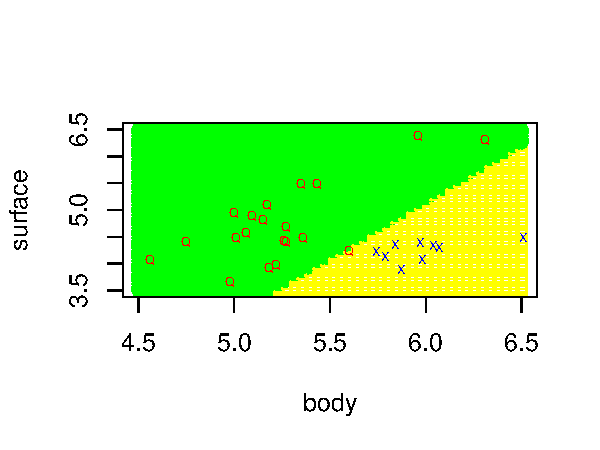
\includegraphics[width=\maxwidth]{figure/unnamed-chunk-3} 

}



\end{knitrout}


\begin{knitrout}
\definecolor{shadecolor}{rgb}{0.969, 0.969, 0.969}\color{fgcolor}\begin{kframe}
\begin{alltt}
\hlcom{# e)}

\hlstd{zm_kanon} \hlkwb{<-} \hlkwd{t}\hlstd{(a)} \hlopt \hlkwd{t}\hlstd{(e[,} \hlnum{2}\hlopt{:}\hlnum{3}\hlstd{])}
\hlstd{prog} \hlkwb{<-} \hlkwd{t}\hlstd{(a)} \hlopt \hlstd{z}

\hlstd{pr} \hlkwb{<-} \hlkwd{ifelse}\hlstd{(}\hlkwd{as.numeric}\hlstd{(zm_kanon)} \hlopt{-} \hlstd{prog} \hlopt{>} \hlnum{0}\hlstd{,} \hlstr{"explosn"}\hlstd{,} \hlstr{"equake"}\hlstd{)}
\hlstd{pr} \hlopt{==} \hlkwd{as.character}\hlstd{(e}\hlopt{$}\hlstd{popn)}  \hlcom{# widac, ze tylko pierwsza zle sklasyfikowana }
\end{alltt}
\begin{verbatim}
##  [1] FALSE  TRUE  TRUE  TRUE  TRUE  TRUE  TRUE  TRUE  TRUE  TRUE  TRUE
## [12]  TRUE  TRUE  TRUE  TRUE  TRUE  TRUE  TRUE  TRUE  TRUE  TRUE  TRUE
## [23]  TRUE  TRUE  TRUE  TRUE  TRUE  TRUE  TRUE
\end{verbatim}
\begin{alltt}
\hlcom{# tabela reklasyfikacji}

\hlstd{pred} \hlkwb{<-} \hlkwd{predict}\hlstd{(l,} \hlkwc{newdata} \hlstd{= e)}\hlopt{$}\hlstd{class}
\hlkwd{table}\hlstd{(popn, pred)}
\end{alltt}
\begin{verbatim}
##          pred
## popn      equake explosn
##   equake      19       1
##   explosn      0       9
\end{verbatim}
\begin{alltt}
\hlcom{# f)}

\hlstd{x0} \hlkwb{<-} \hlkwd{as.data.frame}\hlstd{(}\hlkwd{t}\hlstd{(}\hlkwd{c}\hlstd{(}\hlkwc{body} \hlstd{=} \hlnum{6}\hlstd{,} \hlkwc{surface} \hlstd{=} \hlnum{4}\hlstd{)))}
\hlkwd{predict}\hlstd{(l, x0)}\hlopt{$}\hlstd{class}  \hlcom{# przypisujemy do klasy explosn}
\end{alltt}
\begin{verbatim}
## [1] explosn
## Levels: equake explosn
\end{verbatim}
\end{kframe}
\end{knitrout}


\subsection*{Zadanie 1.3}

\begin{knitrout}
\definecolor{shadecolor}{rgb}{0.969, 0.969, 0.969}\color{fgcolor}\begin{kframe}
\begin{alltt}
\hlcom{# 1.3}

\hlstd{w} \hlkwb{<-} \hlkwd{read.table}\hlstd{(}\hlstr{"http://www.ipipan.eu/~teisseyrep/TEACHING/DM/DANE/wine.data"}\hlstd{,}
    \hlkwc{sep} \hlstd{=} \hlstr{","}\hlstd{)}
\hlkwd{head}\hlstd{(w)}
\end{alltt}
\begin{verbatim}
##   V1    V2   V3   V4   V5  V6   V7   V8   V9  V10  V11  V12  V13  V14
## 1  1 14.23 1.71 2.43 15.6 127 2.80 3.06 0.28 2.29 5.64 1.04 3.92 1065
## 2  1 13.20 1.78 2.14 11.2 100 2.65 2.76 0.26 1.28 4.38 1.05 3.40 1050
## 3  1 13.16 2.36 2.67 18.6 101 2.80 3.24 0.30 2.81 5.68 1.03 3.17 1185
## 4  1 14.37 1.95 2.50 16.8 113 3.85 3.49 0.24 2.18 7.80 0.86 3.45 1480
## 5  1 13.24 2.59 2.87 21.0 118 2.80 2.69 0.39 1.82 4.32 1.04 2.93  735
## 6  1 14.20 1.76 2.45 15.2 112 3.27 3.39 0.34 1.97 6.75 1.05 2.85 1450
\end{verbatim}
\begin{alltt}
\hlkwd{attach}\hlstd{(w)}

\hlcom{# a)}

\hlstd{now} \hlkwb{<-} \hlstd{w[,} \hlkwd{c}\hlstd{(}\hlnum{1}\hlstd{,} \hlnum{2}\hlstd{,} \hlnum{8}\hlstd{)]}
\hlstd{n1} \hlkwb{<-} \hlkwd{length}\hlstd{(}\hlkwd{which}\hlstd{(now[,} \hlnum{1}\hlstd{]} \hlopt{==} \hlnum{1}\hlstd{))}
\hlstd{n2} \hlkwb{<-} \hlkwd{length}\hlstd{(}\hlkwd{which}\hlstd{(now[,} \hlnum{1}\hlstd{]} \hlopt{==} \hlnum{2}\hlstd{))}
\hlstd{n3} \hlkwb{<-} \hlkwd{length}\hlstd{(}\hlkwd{which}\hlstd{(now[,} \hlnum{1}\hlstd{]} \hlopt{==} \hlnum{3}\hlstd{))}
\hlstd{n} \hlkwb{<-} \hlkwd{nrow}\hlstd{(now)}

\hlstd{kol} \hlkwb{<-} \hlkwd{c}\hlstd{(}\hlkwd{rep}\hlstd{(}\hlstr{"red"}\hlstd{, n1),} \hlkwd{rep}\hlstd{(}\hlstr{"blue"}\hlstd{, n2),} \hlkwd{rep}\hlstd{(}\hlstr{"green"}\hlstd{, n3))}
\hlstd{styl} \hlkwb{<-} \hlkwd{c}\hlstd{(}\hlkwd{rep}\hlstd{(}\hlstr{"1"}\hlstd{, n1),} \hlkwd{rep}\hlstd{(}\hlstr{"2"}\hlstd{, n2),} \hlkwd{rep}\hlstd{(}\hlstr{"3"}\hlstd{, n3))}

\hlkwd{plot}\hlstd{(now[,} \hlnum{2}\hlstd{], now[,} \hlnum{3}\hlstd{],} \hlkwc{col} \hlstd{= kol,} \hlkwc{pch} \hlstd{= styl,} \hlkwc{cex} \hlstd{=} \hlnum{0.6}\hlstd{)}
\end{alltt}
\end{kframe}

{\centering 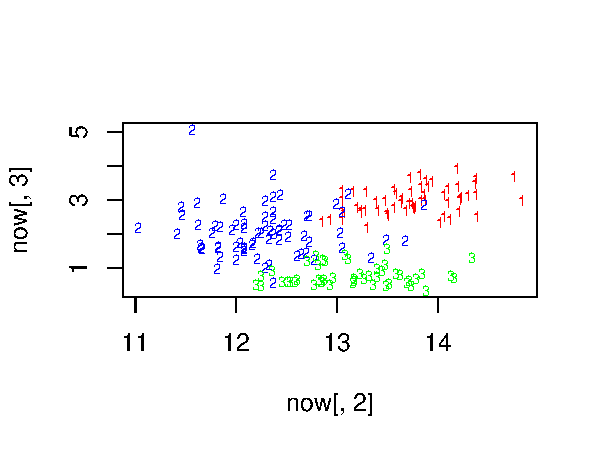
\includegraphics[width=\maxwidth]{figure/unnamed-chunk-5} 

}



\end{knitrout}


\begin{knitrout}
\definecolor{shadecolor}{rgb}{0.969, 0.969, 0.969}\color{fgcolor}\begin{kframe}
\begin{alltt}
\hlcom{# b)}

\hlstd{s} \hlkwb{<-} \hlkwd{sample}\hlstd{(}\hlnum{1}\hlopt{:}\hlstd{n, n}\hlopt{/}\hlnum{2}\hlstd{)}
\hlstd{tren} \hlkwb{<-} \hlstd{w[s, ]}
\hlstd{test} \hlkwb{<-} \hlstd{w[}\hlopt{-}\hlstd{s, ]}

\hlstd{l} \hlkwb{<-} \hlkwd{lda}\hlstd{(V1} \hlopt{~} \hlstd{V2} \hlopt{+} \hlstd{V8,} \hlkwc{data} \hlstd{= tren)}
\hlstd{l_pred} \hlkwb{<-} \hlkwd{predict}\hlstd{(l,} \hlkwc{newdata} \hlstd{= test)}\hlopt{$}\hlstd{class}
\hlstd{(t} \hlkwb{<-} \hlkwd{table}\hlstd{(test}\hlopt{$}\hlstd{V1, l_pred))}
\end{alltt}
\begin{verbatim}
##    l_pred
##      1  2  3
##   1 24  0  0
##   2  5 28  0
##   3  0  3 29
\end{verbatim}
\begin{alltt}
\hlcom{# procent poprawnej klasyfikacji:}

\hlkwd{sum}\hlstd{(}\hlkwd{diag}\hlstd{(t))}\hlopt{/}\hlkwd{nrow}\hlstd{(test)} \hlopt{*} \hlnum{100}
\end{alltt}
\begin{verbatim}
## [1] 91.01
\end{verbatim}
\begin{alltt}
\hlcom{# c)}

\hlstd{x_siat} \hlkwb{<-} \hlkwd{seq}\hlstd{(}\hlnum{11}\hlstd{,} \hlnum{15.5}\hlstd{,} \hlkwc{length.out} \hlstd{=} \hlnum{50}\hlstd{)}
\hlstd{y_siat} \hlkwb{<-} \hlkwd{seq}\hlstd{(}\hlnum{0}\hlstd{,} \hlnum{5.5}\hlstd{,} \hlkwc{length.out} \hlstd{=} \hlnum{50}\hlstd{)}
\hlstd{siatka} \hlkwb{<-} \hlkwd{expand.grid}\hlstd{(}\hlkwc{V2} \hlstd{= x_siat,} \hlkwc{V8} \hlstd{= y_siat)}

\hlstd{l_pred} \hlkwb{<-} \hlkwd{predict}\hlstd{(l, siatka)}\hlopt{$}\hlstd{class}

\hlstd{kol2} \hlkwb{<-} \hlkwd{ifelse}\hlstd{(l_pred} \hlopt{==} \hlstr{"1"}\hlstd{,} \hlstr{"yellow"}\hlstd{,} \hlkwd{ifelse}\hlstd{(l_pred} \hlopt{==} \hlstr{"2"}\hlstd{,} \hlstr{"orange"}\hlstd{,} \hlstr{"white"}\hlstd{))}
\hlstd{styl2} \hlkwb{<-} \hlkwd{ifelse}\hlstd{(l_pred} \hlopt{==} \hlstr{"1"}\hlstd{,} \hlnum{19}\hlstd{,} \hlkwd{ifelse}\hlstd{(l_pred} \hlopt{==} \hlstr{"2"}\hlstd{,} \hlnum{22}\hlstd{,} \hlnum{24}\hlstd{))}
\hlkwd{plot}\hlstd{(siatka,} \hlkwc{pch} \hlstd{= styl2,} \hlkwc{col} \hlstd{= kol2)}
\hlkwd{points}\hlstd{(now[,} \hlnum{2}\hlstd{], now[,} \hlnum{3}\hlstd{],} \hlkwc{col} \hlstd{= kol,} \hlkwc{pch} \hlstd{= styl,} \hlkwc{cex} \hlstd{=} \hlnum{0.6}\hlstd{)}
\end{alltt}
\end{kframe}

{\centering 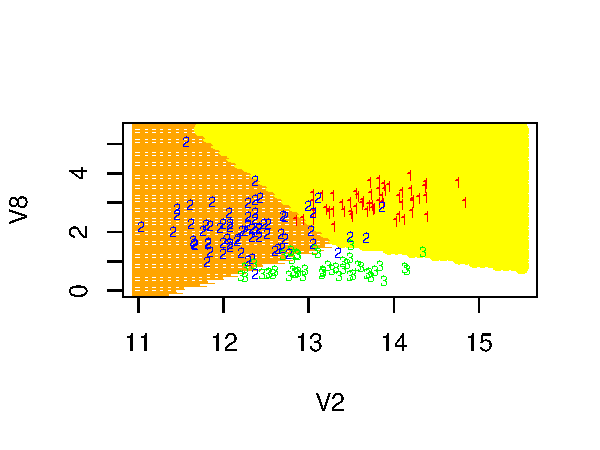
\includegraphics[width=\maxwidth]{figure/unnamed-chunk-6} 

}



\end{knitrout}


\begin{knitrout}
\definecolor{shadecolor}{rgb}{0.969, 0.969, 0.969}\color{fgcolor}\begin{kframe}
\begin{alltt}
\hlcom{# d)}

\hlkwd{library}\hlstd{(}\hlstr{"lattice"}\hlstd{)}

\hlstd{l3} \hlkwb{<-} \hlkwd{lda}\hlstd{(V1} \hlopt{~} \hlstd{V2} \hlopt{+} \hlstd{V8} \hlopt{+} \hlstd{V14,} \hlkwc{data} \hlstd{= tren)}
\hlstd{l3_pred} \hlkwb{<-} \hlkwd{predict}\hlstd{(l3,} \hlkwc{newdata} \hlstd{= test)}\hlopt{$}\hlstd{class}
\hlstd{(t} \hlkwb{<-} \hlkwd{table}\hlstd{(test}\hlopt{$}\hlstd{V1, l3_pred))}
\end{alltt}
\begin{verbatim}
##    l3_pred
##      1  2  3
##   1 24  0  0
##   2  1 31  1
##   3  0  3 29
\end{verbatim}
\begin{alltt}
\hlkwd{sum}\hlstd{(}\hlkwd{diag}\hlstd{(t))}\hlopt{/}\hlkwd{nrow}\hlstd{(test)} \hlopt{*} \hlnum{100}  \hlcom{# wiecej niz w poprzednim modelu}
\end{alltt}
\begin{verbatim}
## [1] 94.38
\end{verbatim}
\begin{alltt}
\hlcom{# e)}

\hlstd{kol} \hlkwb{<-} \hlkwd{c}\hlstd{(}\hlkwd{rep}\hlstd{(}\hlstr{"red"}\hlstd{, n1),} \hlkwd{rep}\hlstd{(}\hlstr{"blue"}\hlstd{, n2),} \hlkwd{rep}\hlstd{(}\hlstr{"green"}\hlstd{, n3))}

\hlkwd{cloud}\hlstd{(w}\hlopt{$}\hlstd{V14} \hlopt{~} \hlstd{w}\hlopt{$}\hlstd{V8} \hlopt{*} \hlstd{w}\hlopt{$}\hlstd{V2,} \hlkwc{screen} \hlstd{=} \hlkwd{c}\hlstd{(}\hlkwc{z} \hlstd{=} \hlopt{-}\hlnum{10}\hlstd{,} \hlkwc{x} \hlstd{=} \hlnum{0}\hlstd{,} \hlkwc{y} \hlstd{=} \hlnum{20}\hlstd{),} \hlkwc{xlab} \hlstd{=} \hlstr{"Alcohol"}\hlstd{,}
    \hlkwc{ylab} \hlstd{=} \hlstr{"Flavonoids"}\hlstd{,} \hlkwc{zlab} \hlstd{=} \hlstr{"Protoline"}\hlstd{,} \hlkwc{col} \hlstd{= kol,} \hlkwc{pch} \hlstd{=} \hlkwd{c}\hlstd{(}\hlkwd{rep}\hlstd{(}\hlnum{1}\hlstd{, n1),}
        \hlkwd{rep}\hlstd{(}\hlnum{20}\hlstd{, n2),} \hlkwd{rep}\hlstd{(}\hlnum{24}\hlstd{, n3)))}
\end{alltt}
\end{kframe}

{\centering 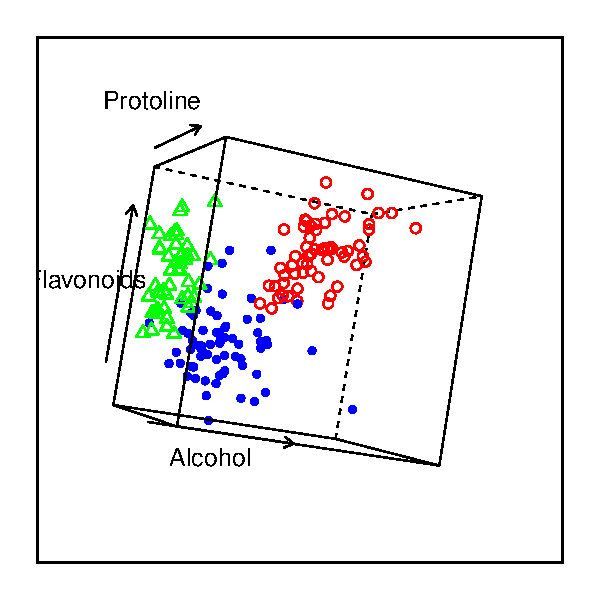
\includegraphics[width=\maxwidth]{figure/unnamed-chunk-7} 

}



\end{knitrout}


\subsection*{Zadanie 1.4}

\begin{knitrout}
\definecolor{shadecolor}{rgb}{0.969, 0.969, 0.969}\color{fgcolor}\begin{kframe}
\begin{alltt}
\hlcom{# 1.4}

\hlcom{# a)}

\hlstd{Y1} \hlkwb{<-} \hlkwd{c}\hlstd{(}\hlkwd{rep}\hlstd{(}\hlnum{1}\hlstd{, n1),} \hlkwd{rep}\hlstd{(}\hlnum{0}\hlstd{, n2} \hlopt{+} \hlstd{n3))}
\hlstd{Y2} \hlkwb{<-} \hlkwd{c}\hlstd{(}\hlkwd{rep}\hlstd{(}\hlnum{0}\hlstd{, n1),} \hlkwd{rep}\hlstd{(}\hlnum{1}\hlstd{, n2),} \hlkwd{rep}\hlstd{(}\hlnum{0}\hlstd{, n3))}
\hlstd{Y3} \hlkwb{<-} \hlkwd{c}\hlstd{(}\hlkwd{rep}\hlstd{(}\hlnum{0}\hlstd{, n1} \hlopt{+} \hlstd{n2),} \hlkwd{rep}\hlstd{(}\hlnum{1}\hlstd{, n3))}

\hlstd{w.lm1} \hlkwb{<-} \hlkwd{lm}\hlstd{(Y1} \hlopt{~} \hlstd{V2} \hlopt{+} \hlstd{V8,} \hlkwc{data} \hlstd{= w)}
\hlstd{w.lm2} \hlkwb{<-} \hlkwd{lm}\hlstd{(Y2} \hlopt{~} \hlstd{V2} \hlopt{+} \hlstd{V8,} \hlkwc{data} \hlstd{= w)}
\hlstd{w.lm3} \hlkwb{<-} \hlkwd{lm}\hlstd{(Y3} \hlopt{~} \hlstd{V2} \hlopt{+} \hlstd{V8,} \hlkwc{data} \hlstd{= w)}

\hlcom{# b)}

\hlstd{p1} \hlkwb{<-} \hlkwd{predict}\hlstd{(w.lm1,} \hlkwc{newdata} \hlstd{= w)}
\hlstd{p2} \hlkwb{<-} \hlkwd{predict}\hlstd{(w.lm2,} \hlkwc{newdata} \hlstd{= w)}
\hlstd{p3} \hlkwb{<-} \hlkwd{predict}\hlstd{(w.lm3,} \hlkwc{newdata} \hlstd{= w)}

\hlstd{razem} \hlkwb{<-} \hlkwd{cbind}\hlstd{(p1, p2, p3)}

\hlstd{p} \hlkwb{<-} \hlkwd{numeric}\hlstd{(n)}
\hlkwa{for} \hlstd{(i} \hlkwa{in} \hlnum{1}\hlopt{:}\hlstd{n) \{}
    \hlstd{p[i]} \hlkwb{<-} \hlkwd{which}\hlstd{(razem[i, ]} \hlopt{==} \hlkwd{max}\hlstd{(razem[i, ]))}
\hlstd{\}}

\hlstd{(t} \hlkwb{<-} \hlkwd{table}\hlstd{(w}\hlopt{$}\hlstd{V1, p))}
\end{alltt}
\begin{verbatim}
##    p
##      1  2  3
##   1 57  2  0
##   2  5 61  5
##   3  0  2 46
\end{verbatim}
\begin{alltt}
\hlkwd{sum}\hlstd{(}\hlkwd{diag}\hlstd{(t))}\hlopt{/}\hlstd{n} \hlopt{*} \hlnum{100}
\end{alltt}
\begin{verbatim}
## [1] 92.13
\end{verbatim}
\end{kframe}
\end{knitrout}


\end{document}
